\documentclass[a4paper]{article}
\usepackage[pdftex]{graphicx}
\usepackage[utf8]{inputenc}
\usepackage{enumerate}
\usepackage{siunitx}
\sisetup{locale=DE}
\usepackage{icomma}
\usepackage{amssymb}
\usepackage{tikz}
\usepackage{href-ul}
\hypersetup{
	colorlinks=true,
	linkcolor=blue,
	urlcolor=blue}
\usepackage{geometry}
\geometry{a4paper, top=15mm, left=15mm, right=15mm, bottom=15mm,
	headsep=10mm, footskip=12mm}

\begin{document}
	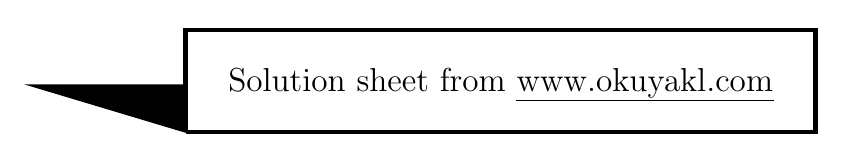
\begin{tikzpicture}(10,3)
		\draw[ultra thick](2,0) --(10,0) -- (10,1.3) --(2,1.3) -- (2,0);
		\draw[fill=black](2,0)-- (0,.6) -- (2,.6) -- (2,0);
		\node at (6,.6) {\large Solution sheet from \href{http://www.okuyakl.com}{www.okuyakl.com}};
	\end{tikzpicture}
	\vspace{0.5 cm}
	
	\begin{minipage}{0.5\textwidth}
		{\bf Task 1. a)}\\
		\includegraphics[width=6 cm]{ikurv235.png}
	\end{minipage}
	\hfill
	\begin{minipage}{0.5\textwidth}
		{\bf Task 1. b)}\\
		The current strength is maximum at the point in time at which the capacitor is discharged. As the current flow continues to decrease, the capacitor charges until the current flow reaches its zero point.
	\end{minipage}
	\vspace{0.5 cm}
	
	\noindent{\bf Task 1. c)}\\
	We consider the total energy as it is combined as magnetic energy in the coil and put:
	$$
	\renewcommand{\arraystretch}{2}
	\begin{array}{rcll}
		W_{tot}&=&{1 \over 2} L \cdot I^2 &|\cdot 2 : I^2\\
		{2 \cdot W_{tot}\over I^2} &=& L \\
		L &=& {2 \cdot \SI{2.9e-3}{\watt} \over (\SI{0.12}{\ampere})^2} &= \SI{0.40}{\henry}
	\end{array}
	$$
	Using the Thomson equation we now get $C$:
	$$
	\renewcommand{\arraystretch}{2}
	\begin{array}{rcll}
		T &=& 2 \pi \sqrt{LC} &| ()^2\\
		T^2 &=& 4 \pi^2 LC & |: 4 \pi^2 L \\
		C &=& { T^2 \over 4 \pi^2 L} \\
		C &=& { (\SI{2.0e-3}{\second})^2 \over 4 \pi \cdot \SI{0.40}{\henry}} \\
		C &=& \SI{2.5e-7}{\farad}&=\SI{0.25}{\micro\farad}
	\end{array}
	$$
	\vspace{0.5 cm}
	
	\noindent{\bf Task 1. d)}\\
	The maximum charge corresponds to the area under the curve during the charging time of the capacitor. Thus $Q_{max}$ is:
	$$
	\renewcommand{\arraystretch}{2}
	\begin{array}{rcll}
		Q_{max} &=& \int\limits_{t_1}^{t_2}I(t)dt\\
		Q_{max} &=& \int\limits_{\SI{0.5}{\milli\second}}^{\SI{1.0}{\milli\second}}\SI{0.12}{ \ampere} \cdot \sin{\left({2\pi \over \SI{2,0}{\milli\second}}\right) \cdot t}dt \\
		Q_{max} &=& \left[\SI{-0.12}{\ampere} \cdot{\SI{2.0}{\milli\second}\over 2\pi} \cos{\left( 2\pi \over \SI{2,0}{\milli\second}\right)\cdot t} \right]_{\SI{0.5}{\milli\second}}^{\SI{1 ,0}{\milli\second}}\\
		Q_{max} &=& \SI{3.8e-5}{\coulomb}
	\end{array}
	$$
	\vspace{0.5 cm}
	
	\noindent{\bf Task 1. e)}\\
	The total energy consists of the energy of the capacitor and the energy of the coil:
	$$
	\renewcommand{\arraystretch}{2}
	\begin{array}{rcll}
		W_{tot} & = & W_{K} + W_{Sp} &| - W_{Sp}\\
		W_{K} & = & W_{ges}- {1 \over 2} LI^2\\
		W_{K} & = & \SI{2.9e-3}{\joule} - {1 \over 2}\cdot \SI{0.40}{\henry} \cdot (\SI{0.090}{\ampere})^2\\
		W_{K} & = & \SI{0.0013}{\joule}
	\end{array}
	$$
	\vspace{0.5 cm}
	
	\noindent{\bf Task 2. a)}\\
	The length of the dipole is half the wavelength:
	$$l_0 = {\lambda \over 2} = {c \over 2 f} = {\SI{3e8}{\meter\over \second}\over 2\cdot \SI{2.5e9}{\hertz} } = \SI{0.06}{\meter} $$
	\vspace{0.5 cm}
	
	\noindent{\bf Task 2. b)}\\
	The Hertzian lattice is only permeable to waves that have a part of the oscillation plane that is perpendicular to it. In the case mentioned, the grid is parallel to the plane of oscillation, therefore it reflects the wave like a conductive surface. The receiving dipole behind the grid does not receive a signal.
	\vspace{0.5 cm}
	
	\begin{minipage}{0.4\textwidth}
		\noindent{\bf Task 2. c)}\\
		\includegraphics[width=5 cm]{hedi235.pdf}
	\end{minipage}
	\hfill
	\begin{minipage}{0.5\textwidth}
		The receiving dipole receives at $0^\circ$ grid rotation 0\%; at $90^\circ$ rotation 100\% of the signal. This suggests that an angle function should be used as a basis. Let the effective length be $l$
		$$l = l_0 \cdot (1-\cos\alpha)$$
		The received power $P$ is proportional to the square of the effective length $l$
		$${P \over P_0} = 100\% \cdot (1-\cos 55^\circ)^2 =18\%$$
		So $D_E$ now receives 18% of the signal.
	\end{minipage}
	\vspace{0.5 cm}
	
	\begin{center}
		\includegraphics[width=7 cm]{../../viecher/eendcomic.pdf}
		
		Here you can go back to the \href{https://www.okuyakl.de/phys/p13schikL235/ae235.pdf}{task sheet}
	\end{center}
	
\end{document}